%---------------------------------------------------------------------
%
%                          Cap�tulo 12
%
%---------------------------------------------------------------------

\chapter{Simulaciones de historias}
\label{cap:Simulaciones}
\begin{FraseCelebre}
	\begin{Frase}
	\end{Frase}
	\begin{Fuente}
	\end{Fuente}
\end{FraseCelebre}

Despu�s de un a�o de trabajo en este cap�tulo se van a exponer los resultados obtenidos durante la elaboraci�n del proyecto.

\section{Flujo de una historia}
Como se ha mencionado anteriormente, el hilo principal de la historia es el secuestro de la \textit{V�ctima} por parte del \textit{Secuestrador}.
Pero lo que se ha introducido son una gran cantidad de factores que hacen que cada simulaci�n el nudo y el desenlace de la historia sea diferente.
Todo esto se consigue gracias al haber introducido elementos en la historia que permiten generar aleatoriedad dentro de las mismas acciones.
Finalmente si se cree que el n�mero de historias diferentes generadas no es suficiente para eso esta todo el SCD que se ha creado.

\section{Historias en funci�n de la parametrizaci�n}
Se ha conseguido con el SCD que si el n�mero de historias que se genera con la parametrizaci�n principal no parece suficiente, cambiando los archivos XML de ``Protagonistas.XML'' ,``Antagonistas.XML'', ``PNJ.XML'', ``Mapa.XML'',``Razas.XML'', ``Objetos.XML'' y ``Frases.XML'' se consiga un nuevo �mbito para generar historias.

\subsection{Historias con parametros m�nimos}
Para las historias m�s reducidas que se pueden generar se necesita que en el archivo ``Protagonistas.XML'' haya como m�nimo un personaje \textit{V�ctima}, un personaje \textit{Allegado} a esta v�ctima y un \textit{Aspirante}, mientras que en el archivo ``Antagonistas.XML'' solo tiene que haber un personaje \textit{Secuestrador}.
Creando un mapa con dos localizaciones es m�s que suficiente para que se genere la historia.
Y por �ltimo se necesita el archivo ``Frases.XML'' que este ser� el m�s extenso de todos.
Para crear esta historia m�nima no son necesarios los archivos ``Razas.XML'', ``PNJ.XML''y ``Objetos.XML''.

\subsection{Ampliando parametros}
Partiendo desde la historia reducida, simplemente incluyendo los archivos que no eran necesarios ya se consiguen nuevas historias o ampliaciones de las historias reducidas.
Por tanto a cuanto mayor cantidad de datos se introduzcan en los archivos XML que afectan a la generaci�n de la historia, la cantidad de historias diferentes que  pueden conseguir crece de forma exponencial.
La siguiente historia se ha generado con una configuraci�n m�nima de al menos un valor para cada apartado posible de cada archivo XML.

\begin{figure}[h]
	\centering
	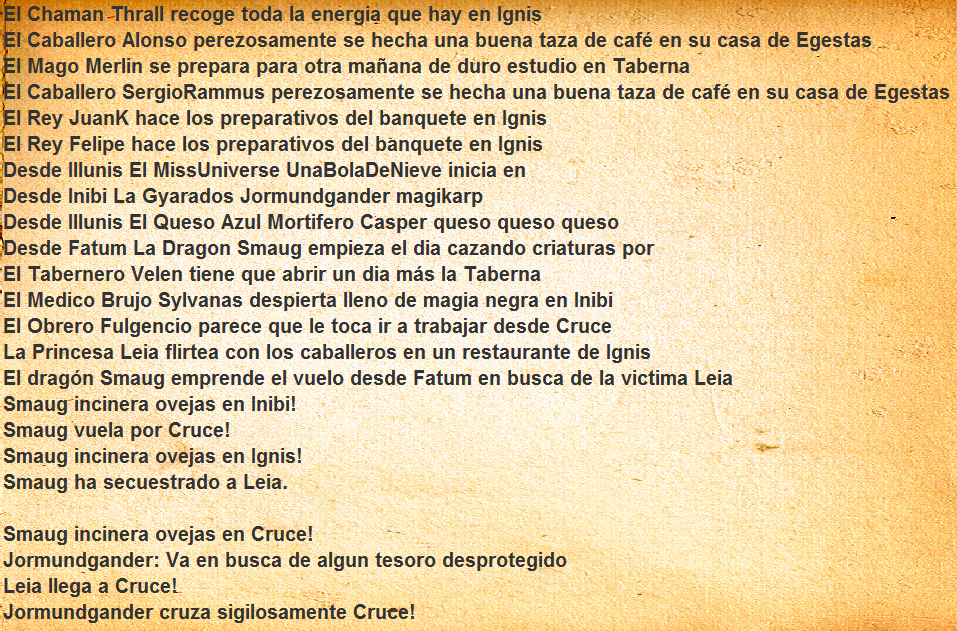
\includegraphics[width=0.8\textwidth]{Imagenes/Historias/EjemploHistoria1}
	\caption{Imagen de ejemplo de una simulaci�n parte 1}
	\label{fig:EjemploHistoria1}
\end{figure}
\newpage
\begin{figure}[h]
	\centering
	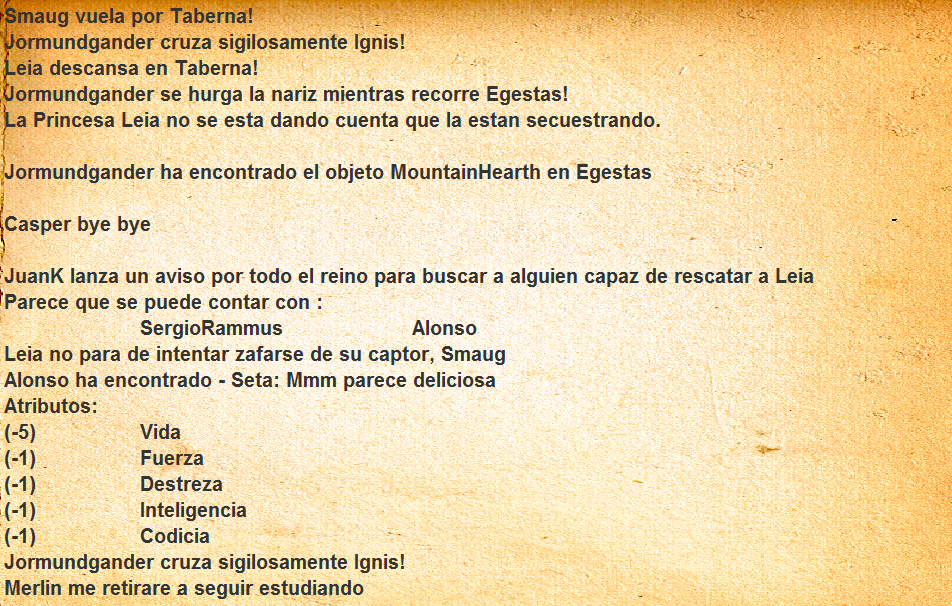
\includegraphics[width=0.8\textwidth]{Imagenes/Historias/EjemploHistoria2}
	\caption{Imagen de ejemplo de una simulaci�n parte 2}
	\label{fig:EjemploHistoria2}
\end{figure}

\begin{figure}[h]
	\centering
	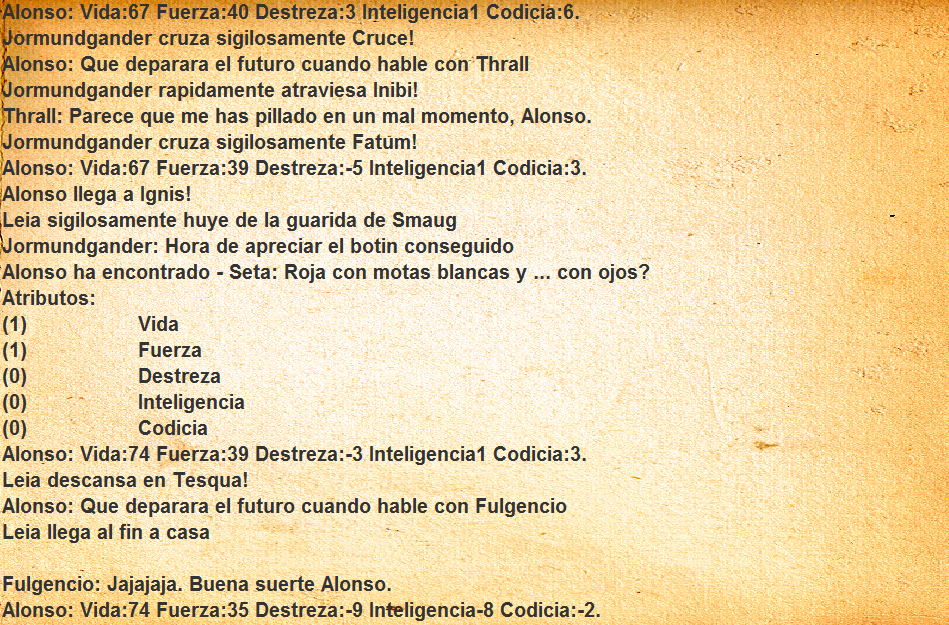
\includegraphics[width=0.8\textwidth]{Imagenes/Historias/EjemploHistoria3}
	\caption{Imagen de ejemplo de una simulaci�n parte 3}
	\label{fig:EjemploHistoria3}
\end{figure}

\begin{figure}[h]
	\centering
	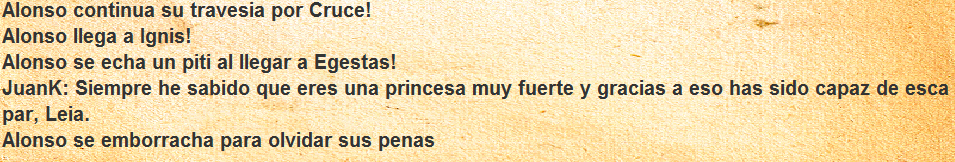
\includegraphics[width=0.8\textwidth]{Imagenes/Historias/EjemploHistoria4}
	\caption{Imagen de ejemplo de una simulaci�n parte 4}
	\label{fig:EjemploHistoria4}
\end{figure}


\newpage
\subsection{Historias famosas}
Adem�s de conseguir multitud de historias tambi�n el sistema permite recrear algunas historias conocidas, como la historia de \emph{Super Mario}, \emph{Zelda} o \emph{Shrek}, simplemente introduciendo los datos en los archivos del SCD (Ver en el siguiente ejemplo).

\subsection{Historia del generador anterior}
Por �ltimo tampoco se quer�a perder la historia desde la que se part�a y se ha realizado la configuraci�n adecuada para los archivos correspondientes para as� guardar la historia desde la que se part�a.


